% !TEX root = ../main.tex
\chapter{Legendre transformation}\label{ch:c18}
\begin{paracol}{2}

\begin{sources}
\begin{tabularx}{\linewidth}{@{}l l L@{}}
\toprule
\textbf{Video} & \textbf{Length} & \textbf{Content}\\
\midrule
\seg{18}{1}{Lecture 18: Legendre transformation (Legendretransformation)} & 1:26:41 & Why a Hamiltonian formulation at all (symmetries and conserved quantities, qualitative solutions, statistical physics, quantum mechanics); the Legendre transformation as the question ``can the information of a function be stored in its slopes?'' (picture of the envelope of tangents, condition $L''\neq0$, definition in three steps and the sign convention); the example $L=\tfrac12mv^2$, and why the transform of a Lagrangian will be $T+V$; the Legendre transformation is its own inverse (proof, and the questions about the conditions); functions of several variables ($2^n-1$ partial transforms); outlook to the Hamilton function in a chart. The recorded date is 26 June 2014; a course evaluation and a break of about 20 minutes sit in the middle (\cref{cn:lt-eval}).\\
\bottomrule
\end{tabularx}

\smallskip
\textbf{Transcript} \file{materials/transcripts/C18-V01.txt} (German YouTube auto-captions, mediocre in the spoken formulas and in the names; formulas reconstructed by recomputing and marked [?] where unsure). The lecturer is Schuller.
\end{sources}

\begin{reading}[Where this lecture sits in the other notes]
Not treated in the other courses.
Continues \cref{ch:c13,ch:c14} (Lagrangian on the tangent bundle) and \cref{ch:c16,ch:c17} (accessible configurations $\mathcal Z$ and charts); the next lecture, \cref{ch:c19}, uses the transformation to build the Hamilton function on the cotangent bundle.
\end{reading}

% ==================================================================
\section{Why a Hamiltonian formulation at all?}\label{sec:lt-why}

``Very good morning, today we come to the part of the lecture on the Hamiltonian formulation of mechanics'' \ts{18}{1}{0:00}. After the Newtonian and the Lagrangian formulation the question is natural: why do we need yet another one? The Lagrangian formulation was ``pretty smart'': one can simply add actions, or Lagrangians, to get composite systems, and constraints were implemented very simply. So what could the aim be? The answer: there is no aim of \emph{more complexity} of the systems; the significance of the Hamiltonian formulation is a different one \ts{18}{1}{0:21}.

\begin{coursenote}[Names in the captions (as said in class)]\label{cn:lt-names}
The auto-captions mangle the key words of this lecture: ``Lagrange'' appears as ``Lacrosse''/``Daniela branche'', ``Hamilton'' as ``hemmelte'' or ``hübsche'', ``Legendre'' as ``Lese(n)dre''/``besondere transformation'', ``Noether'' as ``mütter''/``nur theorien''. In these notes the words are restored from the sense.
\end{coursenote}

\subsection{The phase space: the state of a system}\label{ssec:lt-state}

First recall what the Lagrangian is: a function on the velocity phase space (Geschwindigkeitsphasenraum), technically the tangent bundle $T\mathcal Z$ of the configuration manifold that we prescribe; it determines the dynamics \ts{18}{1}{1:01}. In physics one often speaks of a \emph{phase space} (Phasenraum), whose points give the \emph{state} of a system. The state of a system is ``all the data, all the information that you need to obtain a unique solution curve, if you know the dynamics'': initial position and initial velocity. So the points of the velocity phase space are states. But one can also describe the state differently, namely by the points of the \emph{cotangent bundle}: there the datum is the position together with the \emph{momentum}, and ``the momentum was introduced on the second last problem sheet, so as not to confuse you''; the momentum is an element of the cotangent bundle \ts{18}{1}{1:23}. Hamiltonian mechanics takes place on the cotangent bundle. Given a Lagrangian, we shall find out how to construct from it the Hamilton function $H$, which ``shall please contain all the information that the Lagrangian contains'', and then we get a slightly different formulation \ts{18}{1}{2:04}.

\subsection{Is it worth replacing velocities by momenta? Yes}\label{ssec:lt-worth}

For concrete problems the Lagrangian formulation is excellent (the students have seen it with the double pendulum, \cref{ch:c17}). But the Hamiltonian formulation is ``for everything else, for the theorist a feast'': the best formulation, for example for the following reasons \ts{18}{1}{2:46}.

\begin{enumerate}
  \item \emph{Symmetries and conserved quantities.} One gets the deepest understanding of the relation between the symmetries of a system and its conserved quantities. ``As so often, you were lied to in school'' \ts{18}{1}{3:27}: one learns that momentum, angular momentum and energy are conserved; ``all lies'', in this absoluteness. Momentum conservation holds only in systems with \emph{translation invariance}: if the system is shifted to another point the potential stays the same.
\end{enumerate}

\begin{example}[The falling chalk; the parabolic flight (as said in class)]\label{ex:lt-chalk}
Let the piece of chalk fall: its momentum grows the longer it falls, although ``one thought momentum is conserved''. The reason: in the homogeneous gravitational field, shifting the system horizontally does not change the potential (the system is translation invariant in these two directions), but vertically it does (not translation invariant in this direction). In the parabolic flight, looking at the horizontal coordinates only, the motion is uniform; only in the vertical direction it is accelerated. So momentum conservation holds in the horizontal directions and not in the vertical one \ts{18}{1}{4:09}.
\end{example}
One can show this in the Lagrangian formalism too (``this is the so-called Noether theorem''), but in the Hamiltonian formalism ``you need not even write anything down'': it is directly clear that to every symmetry of a system belongs a conserved quantity; this comes in the next lectures (\cref{ch:c21}) \ts{18}{1}{5:51}. And it is a very deep thing: in quantum mechanics one has no good intuition for the systems any more, but these structures carry over one to one; the relation between symmetries and conserved quantities stays, and must be understood if one wants to understand even the foundations of quantum mechanics \ts{18}{1}{6:12}.

\begin{enumerate}\setcounter{enumi}{1}
  \item \emph{Qualitative solution.} Suppose one is given a very complicated system, and writes down its Lagrangian (as for the double pendulum: ``a huge thing'', one shrank from solving it). Could one simply stare at the Lagrangian and say ``the system will do about this and that''? Whoever could would be taken for a genius by the fellow students. But if one converts the Lagrangian into the Hamilton function and draws its \emph{level lines} over the momentum phase space, then it suffices to stare at this picture, and the system ``will develop roughly so and so'' (``actually exactly, but that is just hand-waving here''): the whole behaviour of the system, qualitatively, at once and without much computation \ts{18}{1}{6:54}. ``And that only the Hamiltonian formalism can do.'' (Done in \cref{ch:c20} and later.)
  \item \emph{Everywhere in later physics.} The Hamiltonian formulation will be central in theoretical physics 2, 3 and 4 (electrodynamics, quantum mechanics, statistical physics): ``an absolutely integral part of the whole formulation of physics as we have it today'' \ts{18}{1}{8:36}.
\end{enumerate}
So: the Lagrangian function is for the practical things, but in the Hamilton function ``you recognise things that are almost always still hidden''. ``We go at it slowly'' \ts{18}{1}{9:18}.

% ==================================================================
\section{The question: store a function in its slopes}\label{sec:lt-question}

The programme of today is the \emph{Legendre transformation} (Legendre-Transformation). Schuller could write in one line how the Hamilton function is obtained from the Lagrangian, give this line the name Legendre transformation, and go on; but the Legendre transformation turns up in all kinds of fields of physics and mathematics, and there is a reason why it always reappears. Instead of writing down the formula he explains the reason: ``this is so important because it plays a huge role again in statistical physics, for example; so important that we use the whole lecture on it; on the other hand it is also a small lecture to take a breath'' \ts{18}{1}{9:39}. It concerns a ubiquitous question in physics, and not only there; at first sight a funny one, but important \ts{18}{1}{11:09}.

\begin{definition}[New concepts: the question that leads to the Legendre transformation]\label{def:lt-question}
Let $L\colon\R\to\R$ be a function (``you can teach this in school shortly after introducing derivatives''). The usual way to understand a function is: to each point of the domain is assigned a function value. \emph{Can one store the information contained in $L$ instead in the following scheme:} to each \emph{slope} $p$ of the curve (the derivative $L'$ at the various points) a \emph{modified} function value $h(p)$ is assigned, i.e.\ in another function $h$, whose arguments are the slopes of $L$? \ts{18}{1}{11:30}
\end{definition}
The set of the arguments $p$ of $h$ is the set of the derivatives of $L$ at the various points. At first sight this is a rather twisted question; ``who comes up with such a thing? Legendre did, he asked for it, and we look at the transformation that he found'' \ts{18}{1}{14:15}.

What is demanded? Not to lose information. ``If we did it so that we lose information we would have missed our goal.'' How do we find out that no information was lost when constructing $h$ from $L$? If we can \emph{reconstruct $L$ from $h$}: then we have taken enough information along \ts{18}{1}{14:57}.

\subsection{The picture: tangent and intercept}\label{ssec:lt-picture}

On the horizontal axis the points $v$ of the domain, on the vertical axis the function values $L(v)$; draw the graph, say convex or concave, as one likes (the lecturer's yellow curve). ``This is information: you know for which $v$ which value; one can code a love letter in it.'' Which information of $h(p)$ do we need at a point $v$, to reconstruct the function value? Look at the slope at $v$, the slope of the tangent. If we know the slope, it suffices to know where the tangent intersects the vertical axis (the \emph{intercept}): with slope and intercept the tangent can be drawn again. So one possibility is to define $h(p)$ via this intercept \ts{18}{1}{15:38}.

\begin{nfigure}
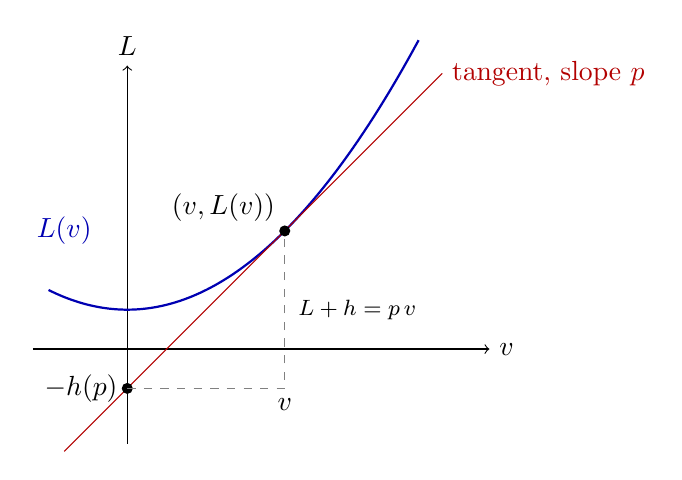
\begin{tikzpicture}[scale=1.0]
  \draw[->] (-1.2,0) -- (4.6,0) node[right] {$v$};
  \draw[->] (0,-1.2) -- (0,3.6) node[above] {$L$};
  \draw[thick,blue!70!black,domain=-1.0:3.7,samples=50,smooth] plot (\x,{0.25*\x*\x+0.5});
  \node[blue!70!black] at (-0.8,1.5) {$L(v)$};
  % tangent at v0=2: L=1.5, p=1, intercept -0.5
  \draw[red!70!black,domain=-0.8:4.0] plot (\x,{1.5+(\x-2)});
  \node[red!70!black,right] at (4.0,3.5) {tangent, slope $p$};
  \fill (2,1.5) circle (2pt); \node[above left] at (2,1.5) {$(v,L(v))$};
  \fill (0,-0.5) circle (2pt);
  \draw[dashed,gray] (0,-0.5) -- (2,-0.5) -- (2,1.5);
  \node[left] at (0,-0.5) {$-h(p)$};
  \node[below] at (2,-0.5) {$v$};
  \node[right,font=\footnotesize] at (2.05,0.5) {$L+h=p\,v$};
\end{tikzpicture}
\caption*{The tangent at $v$ has slope $p=L'(v)$ and meets the $L$-axis at height $-h(p)$ (convention of the lecturer, see below). The right-angled auxiliary triangle gives $p=(L(v)+h(p))/v$.}
\end{nfigure}

But with the intercept and the slope one obtains the whole tangent, and still does not know where on the yellow curve the point lies. So take also another point on the curve, with a slope $p'$ and its intercept: ``imagine that you really do this for all points: you get an \emph{envelope}''. Once the envelope is drawn, you know again what the curve looks like \ts{18}{1}{18:46}.

\begin{coursenote}[The joke of the envelope (as said in class)]\label{cn:lt-joke}
Here Schuller tells a joke (a child comes home and says that all the kids say it has a square head, and the mother answers that it does not have a square head [the captions are garbled]); the point is the \emph{gesture}: one runs a flat hand over something and then everything is clear what the shape is, ``this is exactly the Legendre transformation: you take the hand and move over something, so that the tangent \dots{} you go over it and form the envelope''. ``This is really something from life, running over something with the hand and thereby describing a form'' \ts{18}{1}{20:10}.
\end{coursenote}

\subsection{When does it work? Convexity}\label{ssec:lt-convex}

Can this work for every function? No. Take a function that goes up, then down, then up again, so that the \emph{same slope} occurs at two points, with different intercepts: then for one slope $p$ we would have two values $h(p)$, ``the function $h$ is multivalued, and this is no longer a map''. So it fails for such a function \ts{18}{1}{21:37}.

\begin{nfigure}
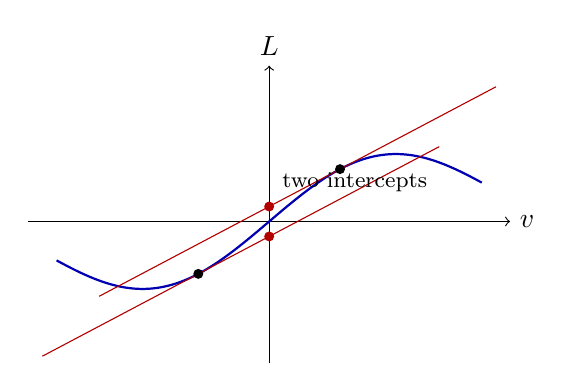
\begin{tikzpicture}[scale=0.9]
  \draw[->] (-3.4,0) -- (3.4,0) node[right] {$v$};
  \draw[->] (0,-2.0) -- (0,2.2) node[above] {$L$};
  \draw[thick,blue!70!black,domain=-3:3,samples=80,smooth] plot (\x,{0.7*sin(\x r)+0.15*\x});
  \draw[red!70!black,domain=-2.4:3.2] plot (\x,{0.739+0.528*(\x-1)});
  \draw[red!70!black,domain=-3.2:2.4] plot (\x,{-0.739+0.528*(\x+1)});
  \fill (1,0.739) circle (2pt); \fill (-1,-0.739) circle (2pt);
  \fill[red!70!black] (0,0.211) circle (2pt); \fill[red!70!black] (0,-0.211) circle (2pt);
  \node[right,font=\footnotesize] at (0.05,0.55) {two intercepts};
\end{tikzpicture}
\caption*{A function with two points of equal slope $p$ and different intercepts: $h(p)$ would be two-valued.}
\end{nfigure}
What is the obvious condition so that no slope occurs twice? A student suggests continuity: no (the function is continuous). Monotonicity: no (a monotone function can have a flat piece, and also monotonically falling or rising functions of $v$ can have repeated slopes). The condition is \emph{convexity}: $L''(v)\neq0$ for all $v$ (for a twice differentiable function). Then $L''$ is either everywhere positive or everywhere negative (otherwise it would have to pass through $0$), i.e.\ the slope always increases (or always decreases), and a slope that always increases never takes the same value twice. Depending on the sign it is called a convexity or a concavity condition; ``this is the condition that one evidently needs on $L$ for this trick with the envelope to work'' \ts{18}{1}{22:59}.

% ==================================================================
\section{From the picture to formulas}\label{sec:lt-formulas}

These are nice pictures, but now they have to be put into formulas, ``which is also quite simple'' \ts{18}{1}{24:45}. Given $L(v)$ and a point $v$. We want to know the slope there: $p:=L'(v)$ (the slope triangle: $\Delta y/\Delta x$). The tangent meets the $L$-axis at some height; we call the \emph{length} of the distance between the axis and the point by $h(p)$ (first naive version). An auxiliary line makes everything clear: the vertical auxiliary segment from the $v$-axis up to the point $(v,L(v))$ has length $L(v)$; the length of the intercept is $h(p)$; so the length of the right-angled triangle's vertical side is $L(v)-h(p)$ and
\begin{equation}\label{eq:lt-slope}
  p\;=\;\frac{L(v)-h(p)}{v}\qquad\text{(first version)}.
\end{equation}
This is how the Legendre transformation is mostly defined in mathematics, ``and also in thermodynamics'' \ts{18}{1}{25:06}. Then the question: why the intercept with the $L$-axis, and not with some other axis, or the five-fold distance, or something squared? The answer: it is a \emph{convention}. ``The convention that is particularly suited in mechanics'' is to call this length not $h(p)$ but $-h(p)$: the quantity to be constructed is $h$, and the positive length is defined as $-h(p)$ (it could just as well land below the axis, then $-h(p)$ would be positive, $h$ negative). ``This sign: do not let anyone talk you out of it, it is pure convention'' \ts{18}{1}{29:02}. The only thing that happens is that we get a plus in \eqref{eq:lt-slope}:
\[
  p\;=\;\frac{L(v)+h(p)}{v},\qquad\text{i.e.}\qquad h(p)\;=\;p\,v-L(v).
\]
Now the right-hand side still depends on $v$; but $p$ can also be computed from its definition as a derivative of the yellow curve, $p=L'(v)$: this gives a second equation, and to make $h$ really a function of $p$ alone, $v$ must be expressed through $p$: ``write $v$ as a function of $p$'', i.e.\ find the \emph{inverse function} of $L'$ \ts{18}{1}{30:47}.

\begin{definition}[New concepts: Legendre transformation (Legendre-Transformation), one variable]\label{def:lt-legendre}
Let $L\colon I\to\R$ ($I\subseteq\R$ an open interval) be twice differentiable with $L''(v)\neq0$ for all $v\in I$. The \textbf{Legendre transform} of $L$ is the function $h$, defined on the set $L'(I)$ of the slopes, obtained in three steps (the lecturer: ``the three boxes, to be learnt by heart and never to be forgotten'' \ts{18}{1}{53:06}):
\begin{enumerate}
  \item \emph{the slope:} $p(v):=L'(v)$;
  \item \emph{the inversion:} solve step 1 for $v$, i.e.\ find the inverse function $v(p)$ of $p(v)$;
  \item \emph{the definition:} $h(p):=p\,v(p)-L\bigl(v(p)\bigr)$.
\end{enumerate}
\end{definition}
\begin{coursenote}[The inverse exists (as said in class)]\label{cn:lt-inverse}
When does the inverse function of $L'$ exist? When $L'$ is injective (surjective one gets always, by restricting the target). By $L''\neq0$ the function $L'$ is strictly monotone, hence injective: this is exactly the multi-valuedness that we saw in the picture \ts{18}{1}{32:32}. A student asks whether the \emph{function} $L$ must be invertible: no (the parabola is not injective), but its \emph{derivative} $L'$ has to be: ``very good intermediate question, because here one must pay attention to which function is meant, $L$ or $L'$'' \ts{18}{1}{34:19}.
\end{coursenote}
The function $h$ is called the \emph{Legendre transform} (Legendre-Transformierte) of $L$ (``and then everybody strokes his head'': the gesture of the envelope) \ts{18}{1}{35:02}.

\begin{aside}[Anecdote on Legendre's portrait (as said in class, not checked)]\label{as:lt-portrait}
There is ``of course the obligatory anecdote'' about Legendre. For over 200 years a portrait of him was printed in all kinds of books and encyclopaedias, showing a man whom one could describe as the most boring theoretical physicist or mathematician imaginable. In 2005 it was found out that this is not Legendre at all, but a French politician of the same surname (``no, I am not drawing comparisons''). People searched for the right picture and found one: there is a single watercolour in a book of the French Academy of Sciences with 73 portraits of members, and ``it is, no joke, the only preserved portrait of the mathematician Legendre''; he looks very grim, ``this must have been shortly before the discovery'' \ts{18}{1}{35:22}. The slides were shown, Schuller adds, only because the evaluation of the course was due that day and point 6.1 of the questionnaire asks about the use of media and projector \ts{18}{1}{37:26}. (As said in class; the date and the details are not checked.)
\end{aside}

% ==================================================================
\section{The example $L=\tfrac12mv^2$, and why the sign}\label{sec:lt-example}

Now a first example, ``and you will see that it is child's play, you have never done anything so easy''. The transition between Lagrange function and Hamilton function \emph{is} a Legendre transformation; for a Lagrangian (a function of many variables) one does not transform with respect to all variables but only with respect to the last ones, the velocities, not the positions: this comes soon \ts{18}{1}{38:04}.

\begin{example}[$L(v)=\tfrac12mv^2$]\label{ex:lt-kin}
Let $L(v)=\tfrac12mv^2$ ($m$ a constant; the notation reminds of the kinetic energy and of the Lagrangian, but for now $L$ is only a function of one real variable). Task (``for example in the first part of the exam''): determine the Legendre transform of $L$.
\begin{enumerate}
  \item $p(v)=L'(v)=mv$.
  \item The inverse (``here the straight line is reflected at the bisector of the angle''): $v(p)=p/m$.
  \item $h(p)=p\,v(p)-L(v(p))=\dfrac{p^2}{m}-\dfrac12m\dfrac{p^2}{m^2}=\dfrac{p^2}{2m}$.
\end{enumerate}
\ts{18}{1}{40:50}
\end{example}
Of course for such a simple exercise one does not think physically about it; but if one does: $L$ is the Lagrangian of a particle in one dimension without potential, i.e.\ the kinetic energy; and $h=p^2/(2m)$ is also the kinetic energy, but written in the momentum $p$ \ts{18}{1}{44:19}. ``Aha, so if we want to relate this to our mechanics, the Lagrangian would perhaps be $T-V$, and then the Hamilton function would be the kinetic energy, \emph{if} $p$ is the momentum.'' Why is it the momentum? A student: ``but the momentum is the derivative of the Lagrangian with respect to the velocity: I defined it so on the problem sheet'' \ts{18}{1}{45:24}; indeed: if one takes the Lagrangian and differentiates it with respect to the velocities (all entries), one obtains the components of the momentum; ``if you wonder why I defined the momentum on the problem sheet as the derivative of the Lagrangian with respect to the velocities, here you have your answer, since the Legendre transform produces for the Hamilton function the kinetic energy''. And, anticipating what will be shown: if the potential energy is $V$ so that $L=T-V$, then the transform of $-V$ carries the sign through, and because of the minus in the definition \[h=T+V,\] the \emph{total energy}. ``Whereas the Lagrangian is the mysterious quantity kinetic minus potential energy, whose meaning is not so obvious [\dots], on passing to the Hamilton function one gets the sum, and one gets the total energy of the system: the Hamilton function has a physical interpretation'' \ts{18}{1}{46:25}. That is the reason for the otherwise arbitrary sign. (``How one finds out such things in research: one has a vague idea, writes down an example that looks like what one wants afterwards, and then starts to observe things.'') \ts{18}{1}{48:07}

\begin{secondary}[Why keep the term $p\,v$? (as said in class)]
After the example a question that Schuller still owes: why define $h(p)=p\,v(p)-L(v(p))$ and not simply $\tilde h(p):=L(v(p))$ (or with a minus)? Also from this one would get something coded in the slopes. But then one loses information: ``the small child with a normal head and the big child with also a normal head have the same envelope'': two functions of the same form but placed differently would give the same $\tilde h$, so $L$ could not be reconstructed from it. ``If you are doing a research project and come by detours to something like this, you do not see at once that it is the Legendre transformation which is asked for; one quickly comes to such an idea, but there information is lost.'' \ts{18}{1}{48:28}--\ts{18}{1}{50:56}.\\
\emph{My check, not said in class:} for $L(v)=\tfrac12(v-a)^2$ one finds $p=v-a$, $v=p+a$ and $\tilde h(p)=\tfrac12p^2$, independent of $a$: a \emph{horizontal} shift of $L$ is lost; the captions say ``how high the curve lies'', but a vertical shift by $c$ would give $\tilde h+c$ and is not lost. With the term $p\,v$ one gets $h(p)=ap+\tfrac12p^2$, which does depend on $a$.
\end{secondary}

\begin{coursenote}[The course evaluation and the break (as said in class)]\label{cn:lt-eval}
At this point (``I would say we make the thousand-men ...'' [the captions are garbled]) the lecturer hands out the evaluation forms and gives 20 minutes: ``you can make a break and fill in the form, and hand it in at the latest at twenty past'' (the form is scanned, evaluated, and he will read the results himself). He asks for participation: valuable feedback on the positive and on the negative sides \ts{18}{1}{51:18}. After the break the lecture continues \ts{18}{1}{52:23}.
\end{coursenote}

% ==================================================================
\section{The back transformation: the Legendre transformation is its own inverse}\label{sec:lt-back}

Still owed: the proof that no information is lost, i.e.\ that from $h$ one can reconstruct $L$. We had: from $L(v)$ we built, in three steps, $h(p)$. The question is whether $h$ contains \emph{all} the information of $L$; the idea is to apply the Legendre transformation once more, now to $h$, and see whether $L$ comes back \ts{18}{1}{52:45}. ``We play a bit with it and make observations'' \ts{18}{1}{54:29}.

\begin{theorem}[The Legendre transformation is an involution]\label{thm:lt-involution}
Let $L$ be as in \cref{def:lt-legendre} and $h$ its Legendre transform. Then
\begin{enumerate}
  \item $h'(p)=v(p)$, \label{it:lt-hprime}
  \item $h''(p)\neq0$ for all $p$ in the domain of $h$, so that $h$ satisfies the hypothesis of \cref{def:lt-legendre}, and
  \item the Legendre transform of $h$ is $L$, with exactly the same three steps (with the roles of $v$ and $p$ exchanged).
\end{enumerate}
\end{theorem}
\begin{proof}
We differentiate $h(p)=p\,v(p)-L(v(p))$ with respect to $p$: the first term by the product rule, the second by the chain rule (outer derivative $L'$, inner derivative $v'(p)$):
\[
  h'(p)\;=\;v(p)+p\,v'(p)-L'\bigl(v(p)\bigr)\,v'(p).
\]
But $L'(v(p))=p$ by the definition of $p(v)$ (step 1) and of its inverse, so the last two terms cancel, and
\[
  h'(p)\;=\;v(p).
\]
(``Aha moment number one: if you differentiate $h$ you get $v$ back, as differentiating $L$ gave $p$'' \ts{18}{1}{56:59}.)
So we can handle $h$ like $L$. Now step 1 for $h$: the new ``slope variable'' is $v:=h'(p)$. For step 2 we need the inverse of $p\mapsto v(p)=h'(p)$, which exists if $h''(p)\neq0$; but $h''(p)=v'(p)\neq0$ since $v$ is the inverse function of the strictly monotone function $L'$ (inverse function theorem: $v'(p)=1/L''(v(p))$) [my addition, not said in class; the lecturer only says: ``technical condition: second derivative of $h$ non-zero'']. The inverse of $h'$ is by construction the function $p(v)=L'(v)$ that we started from \ts{18}{1}{58:22}. Step 3, the definition of the Legendre transform of $h$:
\[
  v\,p(v)-h\bigl(p(v)\bigr)\;=\;v\,p(v)-\Bigl(p(v)\,v-L(v)\Bigr)\;=\;L(v),
\]
using the definition $h(p(v))=p(v)\,v(p(v))-L(v(p(v)))=p(v)\,v-L(v)$. ``We are done'' \ts{18}{1}{58:46}.
\end{proof}
Hence: if $h$ is given, derive it, define $v$ by $v=h'(p)$, invert, and recover $L$: ``these are exactly the same formulas as before, only $v$ and $p$ and $L$ and $h$ exchanged; what I did before with the $L(v)$ I have done now with $h(p)$: a Legendre transformation; I did it twice in a row and am back at $L$ where I started, so no information was lost''. This is also why the minus sign was put into the definition: without it the backward transformation would have a plus sign, and ``this way you always do the same'': \emph{the Legendre transformation is its own inverse}, ``like multiplying by $-1$: twice and you are back'' \ts{18}{1}{59:29}, \ts{18}{1}{1:08:04}. And indeed the hardest step is the inversion; ``everything else is either differentiating or inserting'': one has to find an inverse function once, here it was particularly simple, but it is the hardest step \ts{18}{1}{1:08:48}.

\begin{example}[The back transformation of $h(p)=p^2/(2m)$]\label{ex:lt-back}
Step 1: $v=h'(p)=p/m$. Step 2: the inverse is $p(v)=mv$. Step 3: $L(v)=v\,p(v)-h(p(v))=mv^2-\dfrac{(mv)^2}{2m}=\dfrac12mv^2$, the function we started from: ``at the direct example one sees at once that it works'' \ts{18}{1}{1:05:36}.
\end{example}

\begin{coursenote}[Questions on the conditions (as said in class)]\label{cn:lt-questions}
\begin{enumerate}
  \item A student: the starting point is usually that one has $L$ and computes $h$, \emph{or} has $h$ and should compute $L$. Lecturer: ``I write it so, since you are confronted with the situation of \emph{checking} whether it works backwards.'' The student's follow-up: if one already knows that $h$ came from $L$, can one compute from $h$ directly? One would differentiate $h$ once more and must be careful whether one may cancel; one gets $v'(p)$, and this must not be zero; but a constant $v(p)$ could never arise as the inverse of the function $L'$, because the graph of a constant reflected at the bisector is no function [the captions are garbled here] \ts{18}{1}{1:00:10}.
  \item Another student: $x^3$ does not have a non-zero second derivative everywhere (zero at $0$). Lecturer: true, but then you have the problem anyway: speaking of its inverse (the cube root) one has infinite slopes at $0$, ``and this is also bad'': the conditions are what one needs so that the step back works \ts{18}{1}{1:01:34}.
  \item A student: ``$\geq0$'' is not enough either: there could be a plateau where $L'$ is constant, and the same slope occurs at different points. Lecturer: yes; for instance $L(v)=\alpha v$ gives $p=L'(v)=\alpha$ for all $v$, and one cannot solve for $v$ at all: step 2 fails, ``and this is rubbish and must not be''. A condition that holds only in some regions is not enough; $L''\neq0$ must hold for all $v$ \ts{18}{1}{1:03:23}.
  \item Summary of the lecturer: these examples show that the conditions are not too hard: if they are violated, the path breaks down somewhere \ts{18}{1}{1:07:20}.
\end{enumerate}
\end{coursenote}

% ==================================================================
\section{Functions of several variables}\label{sec:lt-several}

Next: Legendre transforms of functions of several variables, ``I do it for a function of two variables, and from it you know how it goes for all'' \ts{18}{1}{1:09:09}. Take $L\colon\R^2\to\R$, $(v_1,v_2)\mapsto L(v_1,v_2)$. Now one can decide \emph{in which variable} one performs the Legendre transformation. In general, for a function of $n$ variables there are $2^n-1$ different Legendre transforms (strictly speaking one more, the function itself, which is the ``transform with respect to no variable'', ``but then I have done nothing''). For $n=2$: $2^2-1=3$ \ts{18}{1}{1:10:16}.

\begin{definition}[New concepts: partial Legendre transforms of a function of two variables]\label{def:lt-partial}
For $L(v_1,v_2)$ (with the analogue of $L''\neq0$ in each transformed variable; the lecturer does not say what the precise condition is; it is the invertibility of the maps below) define the three functions:
\begin{enumerate}
  \item \emph{transform in the first variable only:} $h_1(p_1,v_2):=p_1\,v_1(p_1,v_2)-L\bigl(v_1(p_1,v_2),v_2\bigr)$;
  \item \emph{transform in the second variable only:} $h_2(v_1,p_2):=p_2\,v_2(v_1,p_2)-L\bigl(v_1,v_2(v_1,p_2)\bigr)$;
  \item \emph{transform in both variables:} $h_{12}(p_1,p_2):=p_1\,v_1(p_1,p_2)+p_2\,v_2(p_1,p_2)-L\bigl(v_1(p_1,p_2),v_2(p_1,p_2)\bigr)$.
\end{enumerate}
Here $p_1(v_1,v_2):=\partial L/\partial v_1$ and $p_2(v_1,v_2):=\partial L/\partial v_2$, and $v_1(p_1,v_2)$, $v_2(v_1,p_2)$, $v_1(p_1,p_2)$, $v_2(p_1,p_2)$ are the inverse functions obtained in the respective step 2 \ts{18}{1}{1:10:58}.
\end{definition}
In the first case ``it is exactly the formula from before, only that this $v_2$ is simply there as the fifth wheel on the cart and nothing happens to it'': only the first variable is replaced by $p_1$ \ts{18}{1}{1:12:48}. Note the point on which the lecturer corrects himself: $p_1$ is a function of \emph{both} $v_1$ and $v_2$ (it is the derivative of $L$ with respect to the first entry, but $L$ still depends on $v_2$), so the inversion gives $v_1$ as a function of $p_1$ \emph{and} $v_2$; ``the inversion depends on more parameters, but this is quite clear from the definition of $p$ as the derivative of a function of two variables'' \ts{18}{1}{1:13:54}. Similarly in the second case, where $v_1$ stays and the inverse $v_2$ depends on $v_1$ and $p_2$ \ts{18}{1}{1:14:56}. In the third case one transforms in both variables: $p_1v_1$ depends on $(p_1,p_2)$ and so on, ``now all variables have been transformed'' \ts{18}{1}{1:16:42}.

For a function of three variables the same holds with $2^3-1=7$ Legendre transforms (the captions say ``77'' [?]); ``and the question is which one you do: it depends on your problem'' \ts{18}{1}{1:17:47}. ``That is all there is to say about the Legendre transformation, at least at this level; the meaning: the form of a function is determined by running over it with the hand, the envelope.'' \ts{18}{1}{1:18:07}

% ==================================================================
\section{Outlook: the Hamilton function in a chart}\label{sec:lt-outlook}

Sixth, an outlook to the next lecture: the Hamilton function as the Legendre transform of the Lagrangian. ``Contrary to our usual habit I do it right away in a chart'', where we can apply at once what we know \ts{18}{1}{1:18:50}.

\begin{definition}[New concepts: the canonical momenta in a chart; the Hamilton function in a chart]\label{def:lt-hamchart}
Let $L$ be a Lagrangian, even one of a system with constraints, ``whatever it is'': in a chart it is a map $L_\omega\colon\R^{2f}\to\R$, $(\alpha^1,\dots,\alpha^f,\beta^1,\dots,\beta^f)\mapsto L_\omega(\alpha,\beta)$ ($f$ the dimension of the manifold of accessible configurations, \cref{cn:pc-f}; $L_\omega=L\circ\xi_\omega^{-1}$ as in \cref{ch:c13}). It is a function of $2f$ variables, and we do \emph{not} want to differentiate with respect to all its components, but define the \textbf{canonical momentum} (kanonischer Impuls; more precisely its components with respect to the chart: ``the momentum covector, or better the momentum-covector components'')
\begin{equation}\label{eq:lt-p}
  p_i(\alpha,\beta)\;:=\;\frac{\partial L_\omega}{\partial\beta^i}(\alpha,\beta)\;=\;\partial_{f+i}L_\omega(\alpha,\beta),\qquad i=1,\dots,f,
\end{equation}
the derivative with respect to the $(f+i)$-th entry, ``all evaluated at all these $\alpha$ and $\beta$''; the abbreviation $\alpha$, $\beta$ stands for the collection of all of them. The \textbf{Hamilton function in the chart} is the Legendre transform of $L_\omega$ with respect to the \emph{last $f$ variables}, the first $f$ remaining untouched:
\begin{equation}\label{eq:lt-H}
  H_\omega(\alpha,p)\;:=\;p_i\,\beta^i(\alpha,p)-L_\omega\bigl(\alpha,\beta(\alpha,p)\bigr),
\end{equation}
where $\beta^i(\alpha,p)$ are the components of the inverse of \eqref{eq:lt-p} with respect to $\beta$: the solution of $p_i=\partial_{f+i}L_\omega(\alpha,\beta)$ for $\beta$ (summation convention over $i=1,\dots,f$; the lecturer's own formula had the indices of the sum garbled, and the students corrected the slips: the $p_i$ in \eqref{eq:lt-H} are the \emph{new variables} and the $\beta^i$ the old ones that have been replaced) \ts{18}{1}{1:19:17}--\ts{18}{1}{1:25:02}.
\end{definition}
Why define these $f$ further quantities at all? ``Because we want them in mechanics, and I need exactly these'' \ts{18}{1}{1:21:23}. The map is the Legendre transformation of \cref{def:lt-partial}, now in $f$ variables at once ($h_{12\dots f}$): the first $f$ entries $\alpha$ are like the fifth wheel on the cart. For the explicit expression of $H$ on the manifold of accessible configurations itself one still has to relate the chart on the tangent bundle with the chart on the new space; ``how exactly, I show you next time; but what you technically must calculate, is this'' \ts{18}{1}{1:22:05}. In the exam:

\begin{coursenote}[What you must be able to do (as said in class)]\label{cn:lt-exam}
``This is what you must do in the exam: I say, set up the Lagrangian for this and that system, do this and do that, and then, as the last subtask: \emph{determine the Hamilton function that belongs to this Lagrangian}'' --- and then you simply do it in the chart: write $L_\omega$, compute the $p_i=\partial L_\omega/\partial\beta^i$, invert them to get $\beta^i(\alpha,p)$, and insert into \eqref{eq:lt-H}. The formula was ``really smeared on the board, I am sorry, but it comes again next time in detail and from a more abstract standpoint; this is just the chart picture'' \ts{18}{1}{1:25:02}. The next meeting is announced (the captions: ``until next Tuesday [?] Monday 8 o'clock, lecture hall H'' [garbled]) \ts{18}{1}{1:26:14}.
\end{coursenote}

% ==================================================================
\section*{Key concepts}
\begin{keyconcepts}
\textbf{Retrieval questions.}
\begin{enumerate}
  \item Which question leads to the Legendre transformation, and how do you check that no information was lost?
  \item State the three steps of the Legendre transformation of $L(v)$. Why must $L''\neq0$ everywhere, and what goes wrong for $L(v)=\alpha v$, and for a function with the same slope at two points?
  \item Compute the Legendre transform of $L(v)=\tfrac12mv^2$, and transform back. What does the sign convention $h=pv-L$ buy you in mechanics?
  \item Prove that $h'(p)=v(p)$ and that the Legendre transformation is its own inverse.
  \item Why is $\tilde h(p)=L(v(p))$ not a good definition?
  \item How many Legendre transforms does a function of $n$ variables have? Write the three transforms of $L(v_1,v_2)$.
  \item How does the Hamilton function in a chart arise from $L_\omega$ (which variables are transformed, which not)?
\end{enumerate}
\textbf{Concepts.}
\begin{itemize}
  \item The question and the envelope (\cref{def:lt-question}, \cref{cn:lt-joke}); convexity $L''\neq0$ (\cref{ssec:lt-convex}).
  \item The three-step definition (\cref{def:lt-legendre}) and the sign convention (\eqref{eq:lt-slope} and below).
  \item The example $L=\tfrac12mv^2\mapsto p^2/(2m)$ (\cref{ex:lt-kin}, \cref{ex:lt-back}).
  \item The Legendre transformation is its own inverse (\cref{thm:lt-involution}); the conditions (\cref{cn:lt-questions}).
  \item Several variables: $2^n-1$ transforms (\cref{def:lt-partial}).
  \item Canonical momenta and the Hamilton function in a chart (\eqref{eq:lt-p}, \eqref{eq:lt-H}), \cref{cn:lt-exam}; next: \cref{ch:c19}.
\end{itemize}
\end{keyconcepts}

\flushside
\end{paracol}
